% $Id: TimeMgr_obj1.tex,v 1.1 2002/08/18 22:43:36 eschwab Exp $

%\section{Object Model}

The core Time Manager Library consists of six object-oriented classes (types)
organized in four layers of inheritance, aggregation and composition,
as shown in Figure 1 below.  The primary classes intended for
direct model use are:

\begin{itemize}
\item ESMF\_TimeInterval
\item ESMF\_TimeInstant
\item ESMF\_Clock
\item ESMF\_Alarm
\item ESMF\_Calendar
\end{itemize}

These directly correspond to, and encapsulate the representation and
behavior of, Time Intervals, Time Instants, Clocks, Alarms, and Calendars,
as specified in the ESMF Time Manager Requirements document.
ESMF\_TimeInterval is independent of any calendar, whereas ESMF\_TimeInstant
is dependent on a calendar type, such as Gregorian or Julian.  Multiple
objects of all these primary classes can be instantiated within a single
application.

There is also one secondary supporting class, not intended for direct
use in model applications.  This is ESMF\_Time.  ESMF\_Time serves as the
base class for both ESMF\_TimeInterval and ESMF\_TimeInstant, capturing
common core time representation and functionality.

ESMF\_Calendar encapsulates all the required calendar types and behavior,
isolating them from Time Instants.  Specific calendar-type objects (e.g.
Gregorian, Julian, no-leap, etc.) can be instantiated from ESMF\_Calendar.
For a given application, it is intended that no more than one calendar
object be instantiated for each calendar type.  The idea is that a calendar
object is analogous to a "wall calendar," serving as a single point of
reference throughout an application.  For example, a single Gregorian
calendar can be instantiated within an application and shared among all
the time instants.

For object integrity, all class data members are private; access is via
public member functions only. The entire ESMF\_Time base class will be
"protected," so that it can only be inherited; it will not be directly
instantiable.

\begin{center}
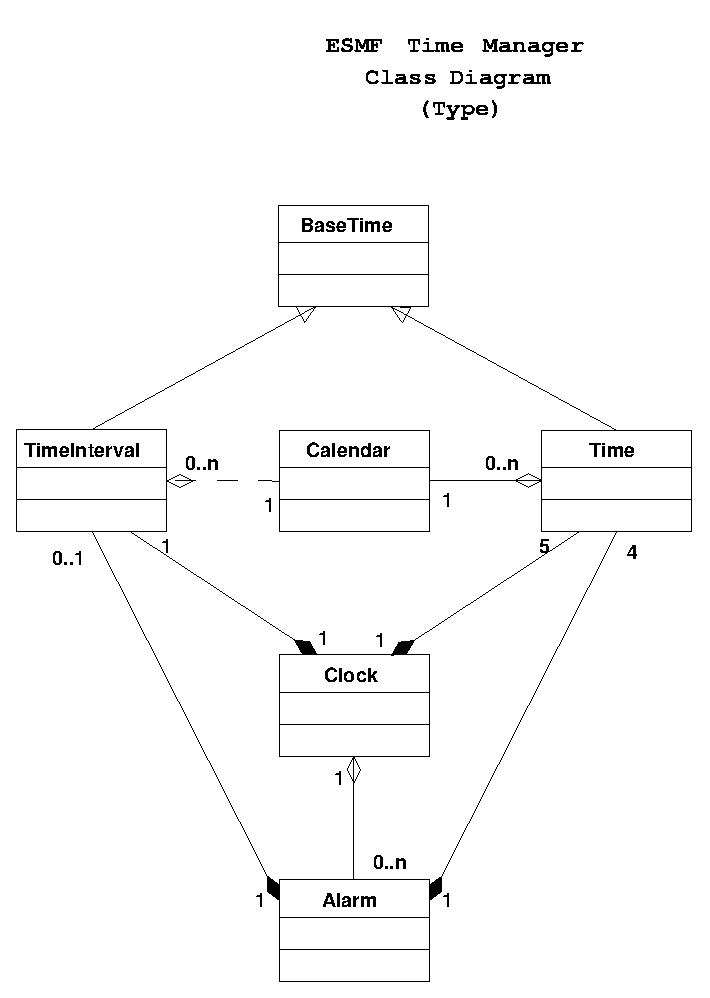
\includegraphics{TimeMgrClass.EPS}
   
Figure 1.  ESMF Time Manager Class Diagram
   
\end{center}
